\label{results}

The search algorithm was allowed to search the space to determine the best material properties.  The resulting response variables can be found in Figure \ref{fig:response_complete}.  Where the blue circular markers indicate material datasets which developed a melt track and the red diamond markers did not have the energy density to produce a melt track.
\begin{figure}[!htb]
	\centering
	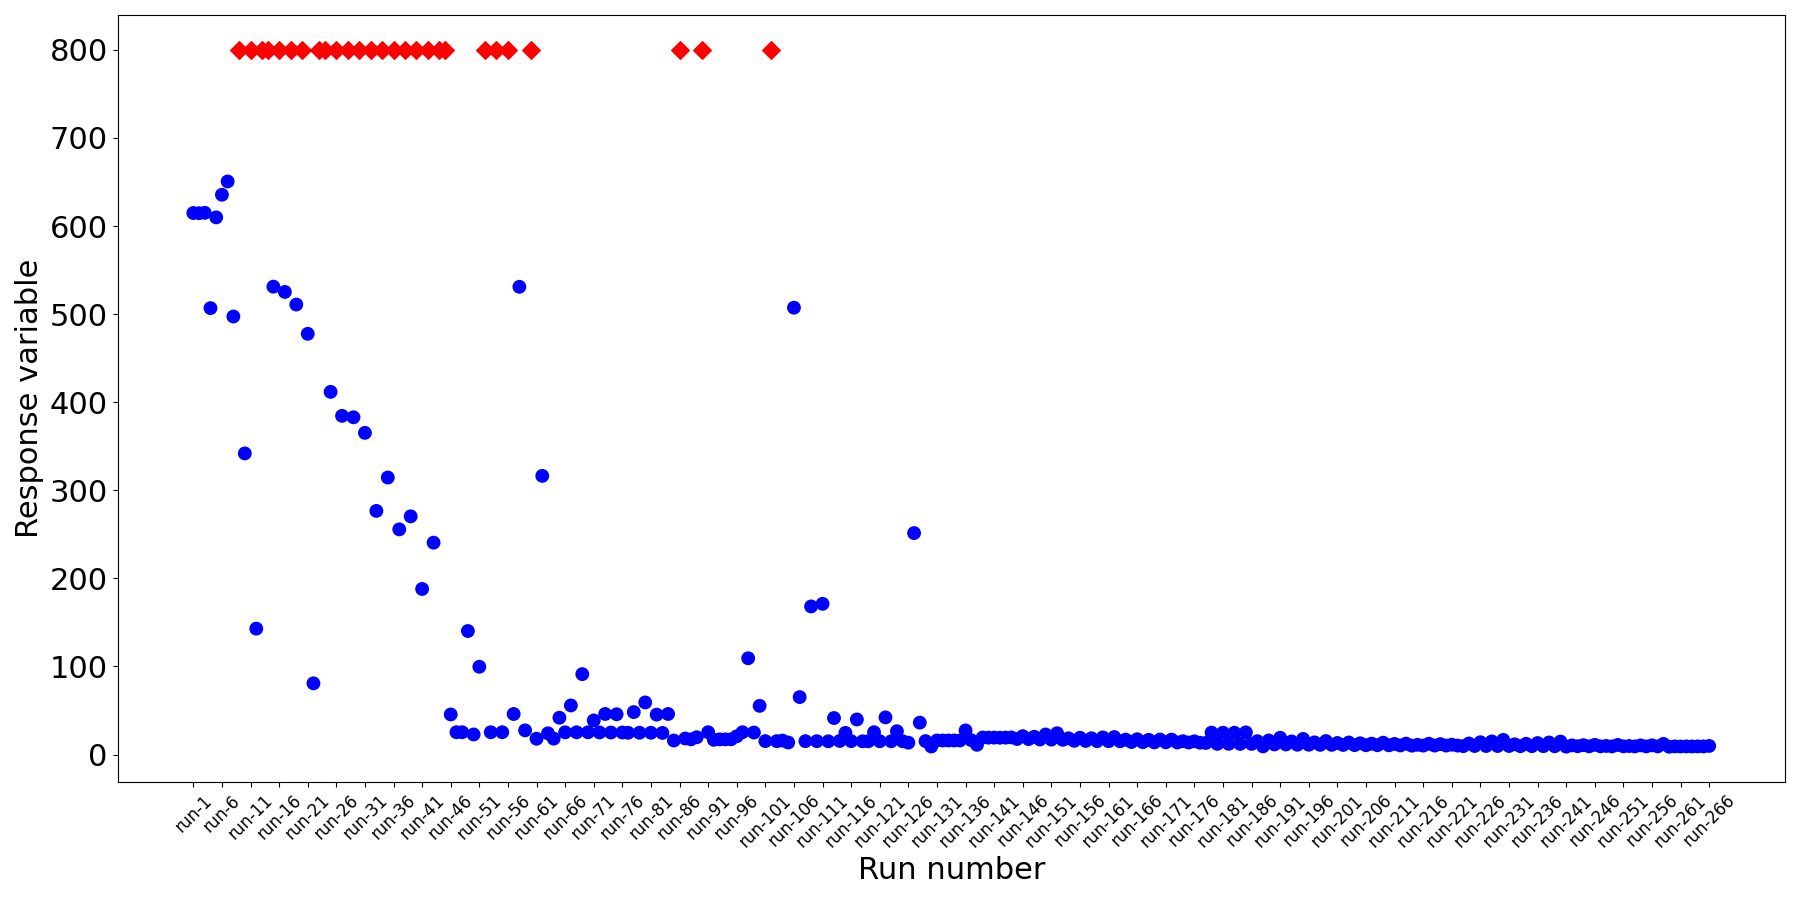
\includegraphics[width=0.75\textwidth]{response_complete}
	\caption{Response variable of the search algorithm for material properties and laser diameter \added{where the blue circle marks developed a melt track and red diamonds did not.}}
	\label{fig:response_complete}
\end{figure}
Due to the vast difference in scales of the initial responses and the final response variables, a new plot was created which has a max Y value of just over 30.  In this plot the blue circular markers are ones which have a response variable less than 30, the green triangle markers are those which completed with a melt track but had response variables greater than 30, and the red diamond markers are those which did not produce a melt track.
\begin{figure}[!htb]
	\centering
	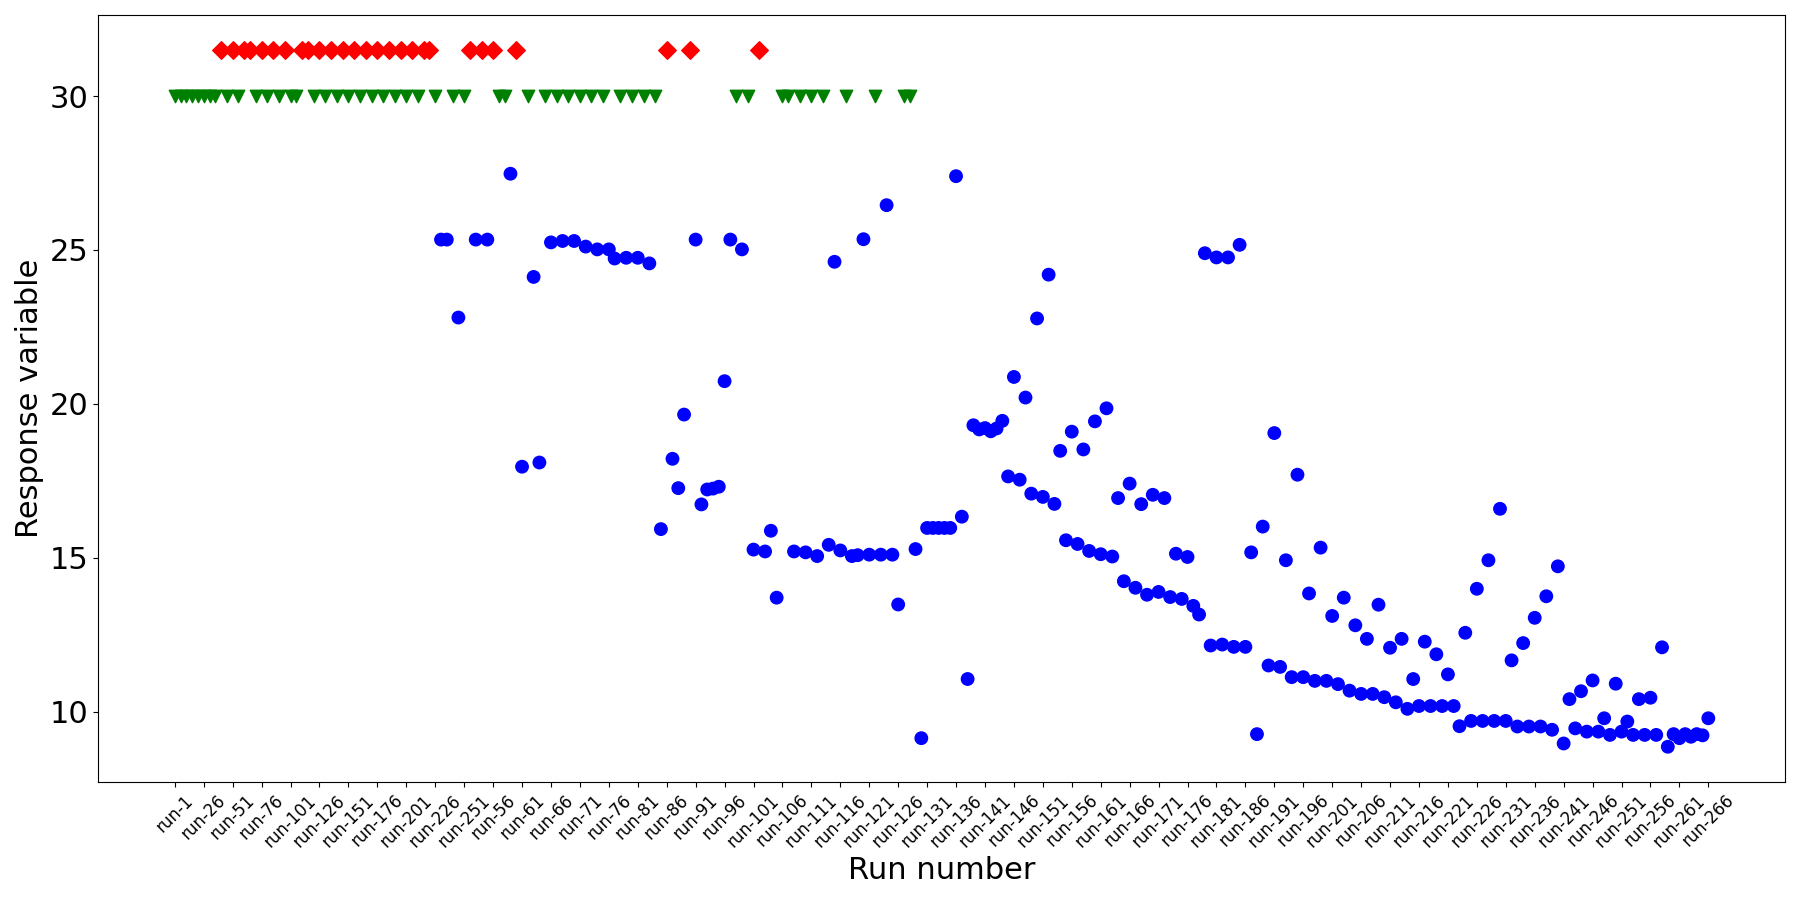
\includegraphics[width=0.75\textwidth]{response_zoomed}
	\caption{Response variable of the search algorithm for material properties and laser diameter with max y axis value of 30 \added{where the blue circle marks developed a melt track, green triangles developed a melt pool but had a response greater than 30, and red diamonds did not develop a melt pool.}}
	\label{fig:response_zoomed}
\end{figure}
In addition to these plots, the error in the width and depth were plotted and can be seen in Figure \ref{fig:tuning_error_complete}.  In these plots, it can be seen that the error in the width is 8.83\% and the error in the depth is 0.03\%.  It is not fully understood why all the error is coming from the width, however, it is theorized that this is a product of the difference in the size of the width vs the depth since the width is nearly triple that of the depth.
\begin{figure}[!htb]\centering
	\begin{subfigure}[c]{0.475\textwidth}\centering
	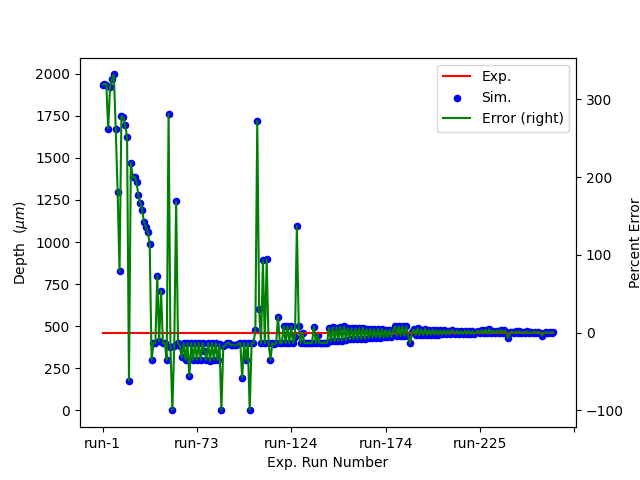
\includegraphics[width=\textwidth]{tuning_error_depth_complete}
	\caption{Melt track depth}
	\label{fig:tuning_error_depth_complete}
	\end{subfigure}\hfill{}
		\begin{subfigure}[c]{0.475\textwidth}\centering
		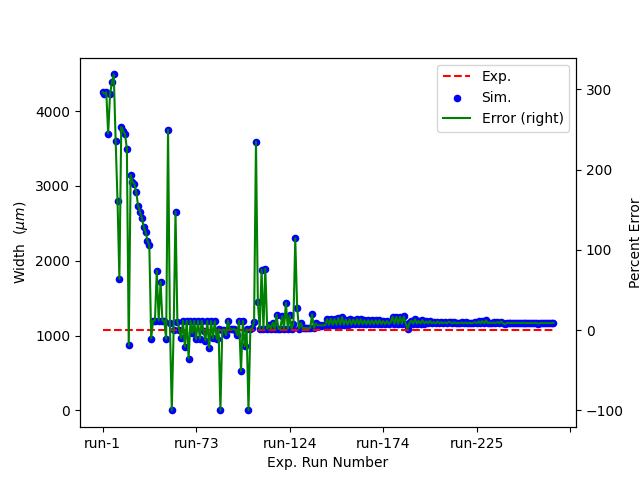
\includegraphics[width=\textwidth]{tuning_error_width_complete}
		\caption{Melt track width}
		\label{fig:tuning_error_width_complete}
		\end{subfigure}
	\caption{Error in the individual runs of the simulations during the \replaced{search}{tuning} algorithm}
	\label{fig:tuning_error_complete}
\end{figure}
\comment{Updated figure captions to include maker explanations \label{rev:figCaptions}}

The search algorithm completed and reduced the combined error from over 600\% when starting from the material properties found in the literature for the generic aluminum material properties, found in Table \ref{tab:starting_mat_prop_complete}, to 9.1\% when using the values found in Table \ref{tab:7000_mat_prop_complete}.
\begin{table}[!htb]
	\centering
	\caption{Optimized \added{Aluminum} material properties and laser diameter dataset for the developed simulation}
	\label{tab:7000_mat_prop_complete}
		\begin{tabular}{|c|c|c|} \hline 
			Property & Material Temp. & Value \\ \hline
			Laser absorption & 880\degree C & 16.8\% \\ \hline
			Laser absorption & 922\degree C & 10.0\%\\ \hline
			Thermal conductivity & 922\degree C & 32.2 $\frac{W}{mK}$\\ \hline
			Thermal conductivity & 1491\degree C & 152.3 $\frac{W}{mK}$\\ \hline
			Specific heat & 733\degree C & 2957.6 $\frac{J}{kgK}$ \\ \hline
			Laser diameter & & 0.864 mm \\ \hline
		\end{tabular}
\end{table}